\documentclass{homework}
\usepackage{lipsum}
\usepackage{cancel}
\usepackage{amsthm}
\usepackage{cleveref}
\usepackage{upgreek}
\usepackage[framed]{mcode}
\usepackage{mathrsfs}
\usepackage{tikz}
\usepackage{units}
\usetikzlibrary{matrix}
\newtheorem{lemma}{Lemma}
\DeclareMathOperator*{\argmin}{arg\,min}

\title{Kevin Joyce}
\course{Math 514 - Inverse Problems - Homework 4}
\author{Kevin Joyce}
\docdate{\today}
\begin{document} 
\newcommand{\figref}[1]{\figurename~\ref{#1}}
\renewcommand{\bar}{\overline}
\renewcommand{\hat}{\widehat}
\renewcommand{\SS}{\mathcal S}
\newcommand{\HH}{\mathscr H}
\newcommand{\mom}{\widetilde}
\newcommand{\mle}{\widehat \Uptheta}
\newcommand{\eps}{\varepsilon}
\newcommand{\todist}{\stackrel{D}\longrightarrow}
\newcommand{\toprob}{\stackrel{p}\longrightarrow}
\newcommand{\TTheta}{\overline{\underline \Theta} }
\newcommand{\del}{\partial}
\newcommand{\approxsim}{\overset{\cdotp}{\underset{\cdotp}{\sim}}}

Codes for each problem are available at \url{https://github.com/kjoyce/inverse_problems/tree/master/homework04/codes}

\begin{longproblem} 
Bardsley 2.9. In exercise 1.2, you were asked to modify \texttt{Deblur1d.m} so that the convolution kernel
$$
  a(s) = \begin{cases}
  100s + 10,  &-\frac 1{10} \le s < 0,\\
  -100s + 10, &0\le s \le \frac 1{10},\\
  0,	      &\text{otherwise}
  \end{cases}
$$
is used instead to define $\vect A$.

\subproblem{ Use Tikhonov regularization together with GCV and L-curve to reconstruct $\vect x$ from observations $\vect b$.  What is the optimal regularization parameter $\alpha$ in each case?  Which gives the better reconstruction in your opinion?}
\begin{solution} 
The reconstructed solutions are given in the following figure with the optimal regularization parameter (based on the data) indicated in the legend:
\begin{center}
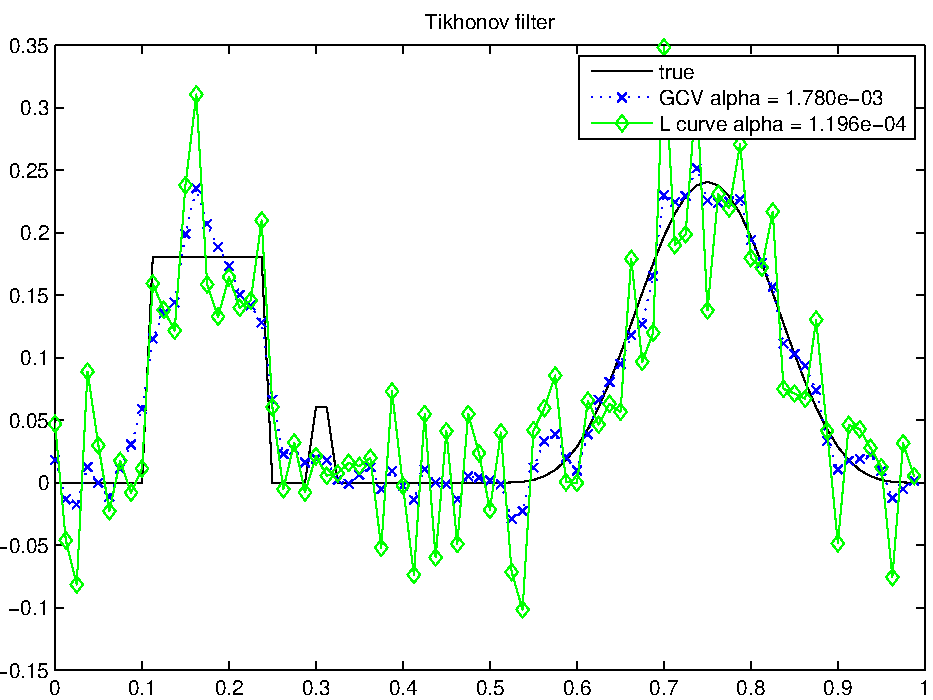
\includegraphics[width=.4\textwidth]{29a_reconstruction.pdf}
\end{center}
The reconstructions are nearly indistinguishable, however GCV seems to be ``closer'' to the true solution. 
\end{solution}

\subproblem{Use TSVD regularization together with UPRE and DP to reconstruct $\vect x$ from observations $\vect b$.  What is the optimal regularization parameter $k$ in each case?  Which gives the better reconstruction in your opinion?}
\begin{solution} 
The reconstructed solutions are given in the following figure with the optimal regularization parameter (based on the data) indicated in the legend:
\begin{center}
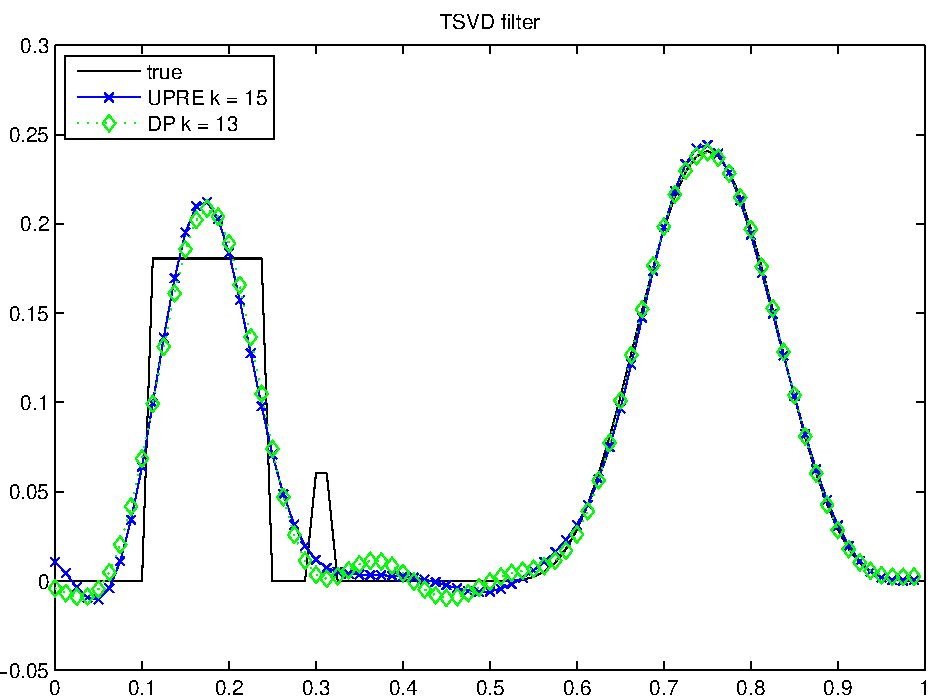
\includegraphics[width=.4\textwidth]{29b_reconstruction.pdf}
\end{center}
The reconstructions are practically indistinguishable, and on several runs the selection methods give the same parameter.  In my opinion, UPRE gives a better reconstruction. 
\end{solution}
\end{longproblem}

\problem{Bardsley 3.1. Modify \texttt{OnedDeblurBCs.m} so that it implements GCV and UPRE regularization parameter selection methods.  How do these parameter selection methods perform in terms of the visual quality of the regularized reconstructions?}
\begin{solution}
\begin{minipage}{.45\textwidth}
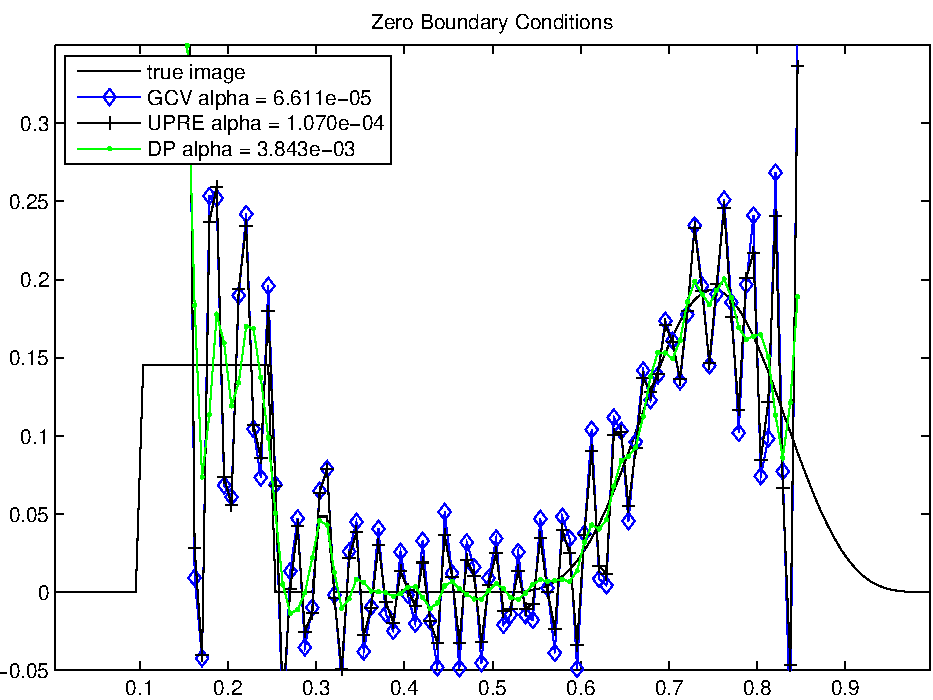
\includegraphics[width=\textwidth]{zero_bc_recon.pdf}
\end{minipage} 
\begin{minipage}{.45\textwidth}
The solutions with zero boundary conditions perform poorly especially near the boundary due to the inappropriate condition.
Note that in this particular reconstruction GCV and UPRE produced nearly identical parameters.
\end{minipage}
\noindent
\begin{minipage}{.45\textwidth}
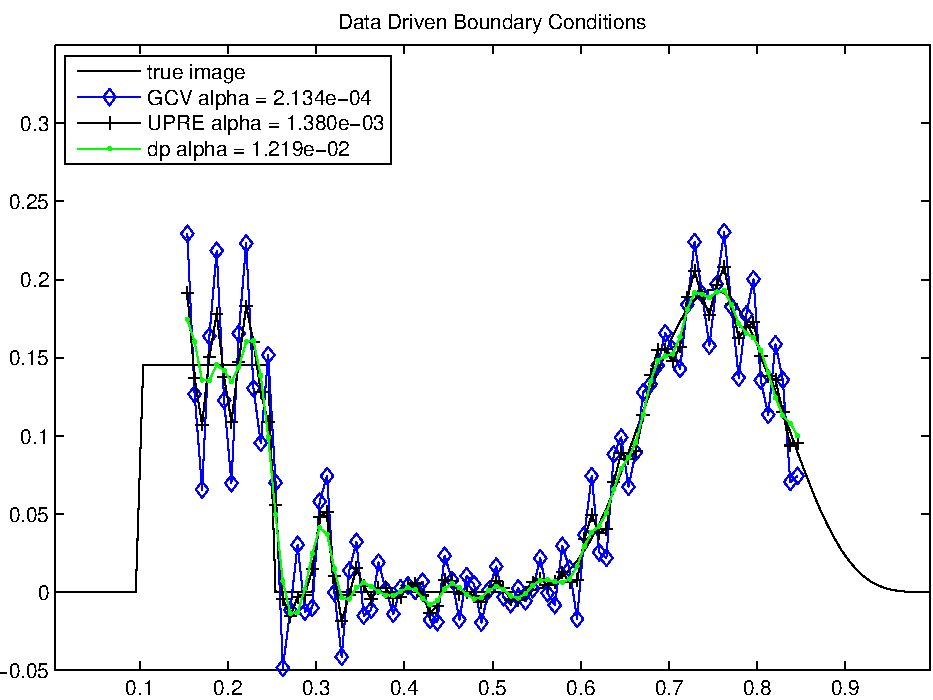
\includegraphics[width=\textwidth]{data_bc_recon.pdf}
\end{minipage} 
\begin{minipage}{.45\textwidth}
In these reconstructions, it appears that GCV is provides less agressive filtering parameters than UPRE.  Note the improvement from the zero boundary reconstruction in that the small feature to the right of the square wave would be difficult to detect with GCV and UPRE in the previous case.  Whereas in the data driven boundary conditions, each parameter selection method reconstructs a solution that has the feature.
\end{minipage}

\end{solution}
\newpage
\problem{Bardsley 3.5. Use the Kronecker product properties 
\begin{align*}
  (\vect A \otimes \vect B)^T &= \vect A^T \otimes \vect B^T \tag{3.12}\\
  (\vect A \otimes \vect B)^\dagger &= \vect A^\dagger \otimes \vect B^\dagger \tag{3.13}\\
  (\vect A \otimes \vect B)(\vect C \otimes \vect D) &= \vect {AC} \otimes \vect{BD}\tag{3.14}\\
\end{align*}
to prove 
\begin{equation}
\vect x_{\mathrm{LS}} = ((\vect A^T_1\vect A_1)^{-1} \vect A_1^T)\otimes((\vect A^T_1\vect A_1)^{-1} \vect A_1^T)\vect b, \tag{3.15}
\end{equation} and 
\begin{equation}
\vect A = (\vect U_1 \otimes \vect U_2)(\vect \Sigma_1\otimes \vect \Sigma_2)(\vect V_1 \otimes \vect V_2)^T. \tag{3.16}
\end{equation}}
\begin{solution}
This solution to due to Cody Palmer.

Recall that the least squares solution is given by left multiplication of the psuedo inverse.  I.e.
\begin{align*}
  \vect A^\dagger \vect b &= (\vect A_1 \otimes \vect A_2)^\dagger \vect b \\
  &= (\vect A_1^\dagger \otimes \vect A_2^\dagger)\vect b&\text{ by (3.13)}\\
  &= ((\vect A^T_1\vect A_1)^{-1} \vect A_1^T)\otimes((\vect A^T_1\vect A_1)^{-1} \vect A_1^T)\vect b.
\end{align*}

For (3.16), we write $\vect A_1 = \vect U_1\vect \Sigma_1 \vect V_1^T$ and $\vect A_2= \vect U_2\vect \Sigma_2 \vect V_2^T$.  Then
\begin{align*}
  \vect A &= \vect(A_1 \otimes \vect A_2) \\
  &= (\vect U_1\vect \Sigma_1 \vect V_1^T)\otimes(\vect U_2\vect \Sigma_2 \vect V_2^T)\\
  &= (\vect U_1 \otimes \vect U_2)(\vect \Sigma_1\otimes \vect \Sigma_2)(\vect V_1^T \otimes \vect V_2^T)&\text{ by (3.14),}\\
  &= (\vect U_1 \otimes \vect U_2)(\vect \Sigma_1\otimes \vect \Sigma_2)(\vect V_1 \otimes \vect V_2)^T&\text{ by (3.12).}
\end{align*} 
\end{solution}

\problem{Bardsley 3.6a. Derive the formulas for GCV analogous to (3.18).  Add lines of code to \texttt{Deblur2dSeparable.m} so that it implements GCV.}
\begin{solution}
  The GCV curve for the separable kernal $\vect A_1\otimes \vect A_2$ is given by
  $$
  G(\alpha) = \left(\sum_{i,j=1}^n \frac{\alpha^2([\vect U_1^T \vect B\vect U_2]_{ij})^2}{([\vect \sigma_1\vect \sigma_2^T]_{ij}^2 + \alpha)} \right) \left/ \middle( m - \sum_{i,j=1}^n\frac{[\vect \sigma_1\vect \sigma_2^T]_{ij}^2}{[\vect \sigma_1\vect \sigma_2^T]_{ij}^2 + \alpha} \right).
  $$
  The following line of code implements the GCV curve:
  \lstinputlisting[language=matlab, firstline=46, lastline=46]{codes/Deblur2dSeparable.m}

  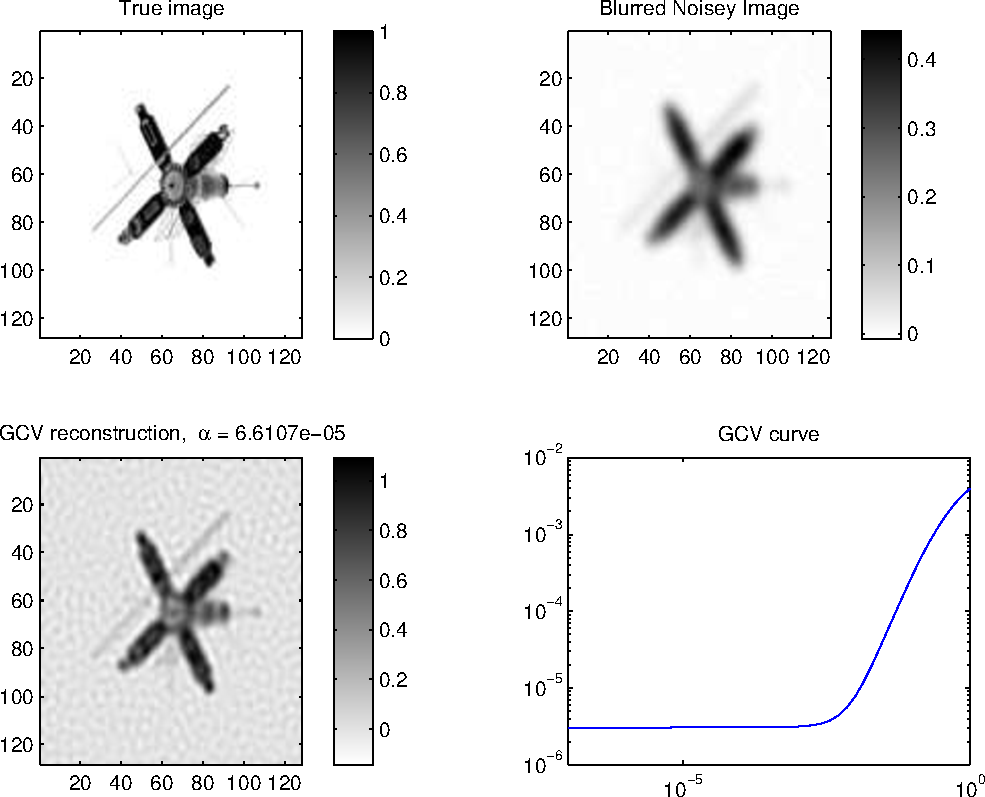
\includegraphics[width=.75\textwidth]{images.pdf}

\end{solution}
\end{document} 
